\documentclass[final,a4paper,10pt]{article}


\usepackage[top=2.3cm, bottom=2.2cm, left=2.8cm, right=2.3cm]{geometry}
%\parskip=5mm
\usepackage{lmodern}
\usepackage[utf8]{inputenc}

\usepackage{mathtools}
\usepackage{graphicx}
\usepackage{fancyhdr} % activamos el paquete
\usepackage{subfig}

\usepackage[all]{xy}
\usepackage[hidelinks]{hyperref}   % use for hypertext links, including those to
\usepackage{xcolor}
\hypersetup{colorlinks, linkcolor={red!50!black},citecolor={blue!50!black},urlcolor={blue!80!black}}
\usepackage{units}
\usepackage{url}
\usepackage{fancybox}
\usepackage{amssymb}
\usepackage{multirow}
\usepackage{float}
\usepackage{bigints}
\usepackage{array}
\usepackage{cancel}
\usepackage{braket}
\usepackage{listings}
\setlength{\parskip}{\baselineskip}
\numberwithin{equation}{section}
\numberwithin{figure}{section}
\numberwithin{table}{section}


\author{Sonia López Bravo}
\title{\bf{Explaining Quantum Physics on Youtube}}
\date{}

\begin{document}
\maketitle

\pagestyle{fancy}
\rhead{}
\lfoot{} % imagen centro del pie
\cfoot{}
\rfoot{\thepage} % texto derecha del pie
\renewcommand{\headrulewidth}{0pt} % grosor de la línea del pie
\renewcommand{\footrulewidth}{0.4pt} % grosor de la línea del pie
\renewcommand{\tablename}{Tabla}
\section{Why science popularization?}
Science is valued by society because the application of scientific knowledge helps to satisfy many basic human needs and improve living standards. Finding a cure for cancer and a clean form of energy are just two topical examples.


To have a society that is each day better, more advanced and well-educated. Right to knowledge 
To avoid misconceptions and the increase of pseudoscience.
A society which regards the importance of science, technology and innovation for development.

In this work we study how 
Scientists often justify their work using these and similar arguments—currently linked to personal health and longer life expectancies, technological advancement, economic profits, and/or sustainability—in order to secure funding and gain social acceptance.
\section{The process of making videos}
Make a short video using animation explaining concepts about entanglement and quantum info (e.g.
quantum communication) for an untrained audience. The point is to make quantum physics in
particular (and science in general) attractive and accessible. This video will be in cooperation with a
scientific youtuber who has over 1.6 million of subscribers, Quantum Fracture.

Once we have chosen the topic of our video and we have consulted the corresponding literature, we can start to make the video. 
\begin{enumerate}
\item \textit{Script:} write the script using always the literature as resouce, in our case \textit{What can we learn about quantum physics from a single qubit}. The point is to make quantum physics in particular (and science in general) attractive and accessible for a likely untrained audience, for that reason the video must be short, no more than 10 minutes, the language must be adapted but being precise, and
\item \textit{Storyboard:} Draw the storyboard following the script. This will help us on the production step
\item \textit{Production:} Make the video using animation in After Effects (Adobe). The pictures must be explanatory but also beautiful
\item \textit{Post-production:} Add sound effects
\end{enumerate}

\section{How to validate learning}
Our aim is to explain quantum physics using animation video on YouTube, once it is uploaded to the YouTube channel we have to check the impact on the audience. YouTube provides some basic features, such as the number of views, the number of likes, the comments section and other more interesting ones, such as the audience engagement.

Nevertheless, this is not enough to see whether the video really works and it is functional for teaching quantum physics. For that reason we ask people to fill in two surveys, one before watching the video and one after. 

\section{Results}
Surveys were available online for a week, since 9th to 17th May 2019, and there were 59807 participants of different ages and scientific knowledge. 

We can start to study the observable ages of all participants as statistical population. When studying a population, it is often convenient to use population parameters, numbers that provide a summary of the statistical features of the population. These are central tendency parameters (mean, median, and mode being the most important) and dispersion parameters (range and standard deviation).

Participants are all between the ages of 5 and 75, nevertheless they are centered between 14 and 40 and the mean is 21. In \ref{fig:age}, where is represented the age dispersion, we can see that the mode is 18, with a second pique at 22 and the median is 19



Among the survey participants
\begin{figure}[H]
    \begin{center}
        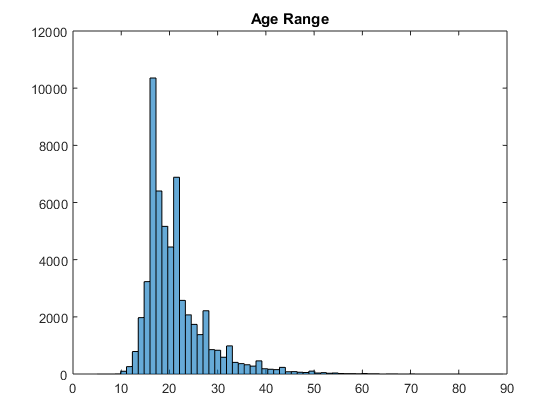
\includegraphics[scale=0.6]{Ages_V1.png}
    \end{center}
    \caption{\footnotesize Bar chart of dispersion of ages.}
    \label{fig:age}
\end{figure}

\begin{figure}[H]
 \centering
  \subfloat[]{
   \label{fig:CQ1}
    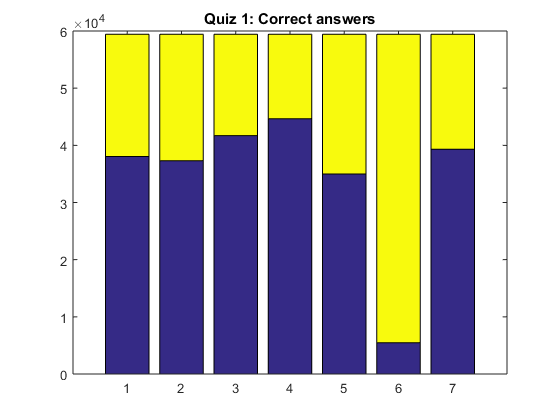
\includegraphics[width=0.5\textwidth]{CorrectQ1.png}}
  \subfloat[]{
   \label{fig:CQ2}
    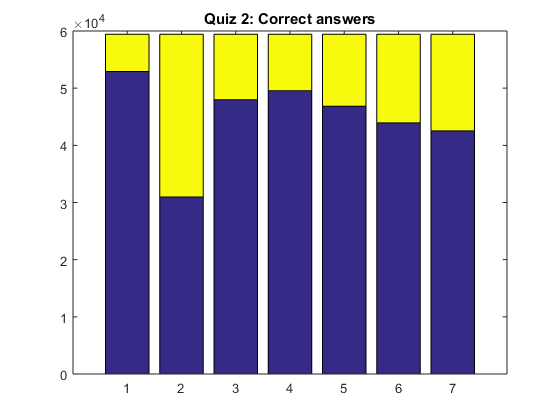
\includegraphics[width=0.5\textwidth]{CorrectQ2.png}}
    \caption{\footnotesize Correct answers to both surveys beside total answers.}
 \label{fig:correct}
\end{figure}


\begin{figure}[H]
 \centering
  \subfloat{
   \label{fig:E1P1}
    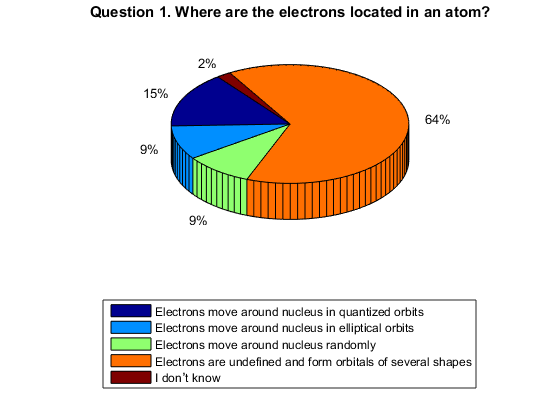
\includegraphics[width=0.45\textwidth]{E1P1_V1.png}}
  \subfloat{
   \label{fig:E1P2}
    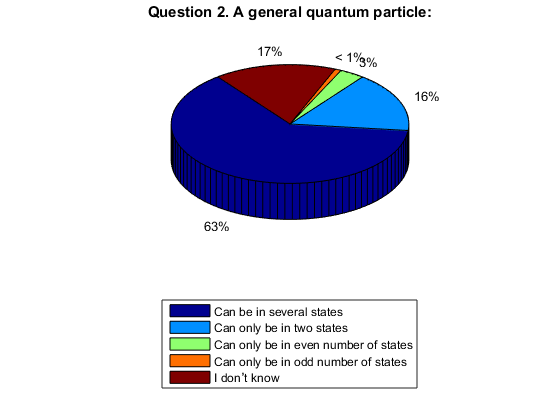
\includegraphics[width=0.45\textwidth]{E1P2_V1.png}}
    \\
     \subfloat{
   \label{fig:E1P3}
    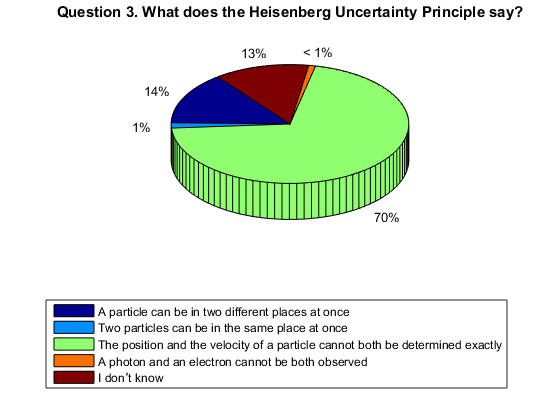
\includegraphics[width=0.45\textwidth]{E1P3_V1.png}}
     \subfloat{
   \label{fig:E1P4}
    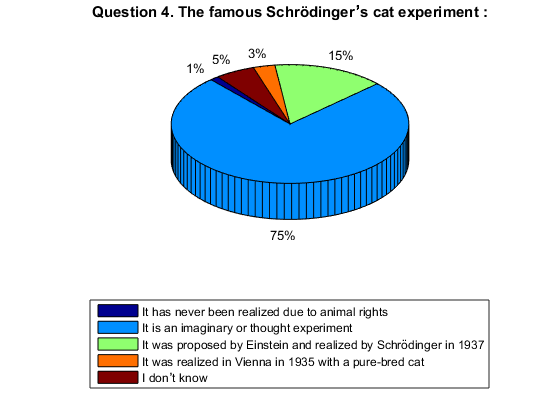
\includegraphics[width=0.45\textwidth]{E1P4_V1.png}}
    \\
    \subfloat{
   \label{fig:E1P5}
    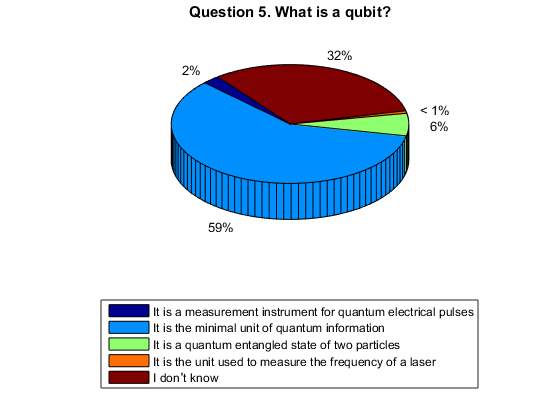
\includegraphics[width=0.45\textwidth]{E1P5_V1.png}}
     \subfloat{
   \label{fig:E1P6}
    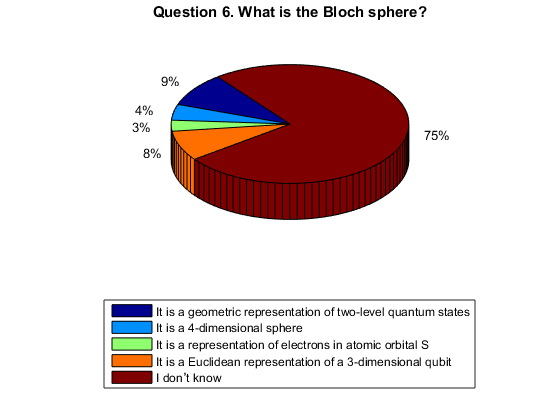
\includegraphics[width=0.45\textwidth]{E1P6_V1.png}}
    \\
     \subfloat{
   \label{fig:E1P7}
    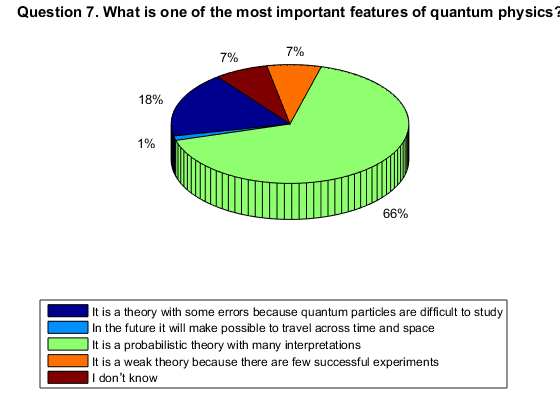
\includegraphics[width=0.45\textwidth]{E1P7_V1.png}}
     \caption{\footnotesize Answers Survey 1: Before watching the video.}
 \label{fig:encuesta1}
\end{figure}


\begin{figure}[H]
 \centering
  \subfloat{
   \label{fig:E2P1}
    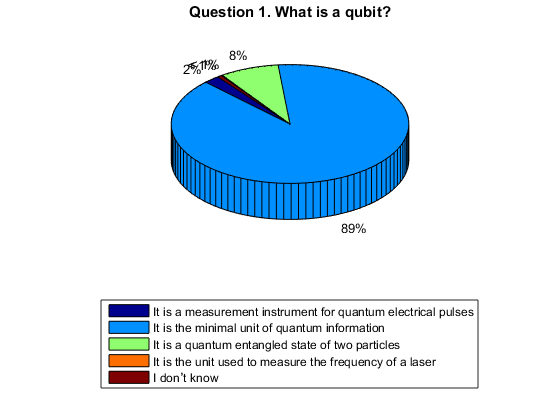
\includegraphics[width=0.45\textwidth]{E2P1_V1.png}}
  \subfloat{
   \label{fig:E2P2}
    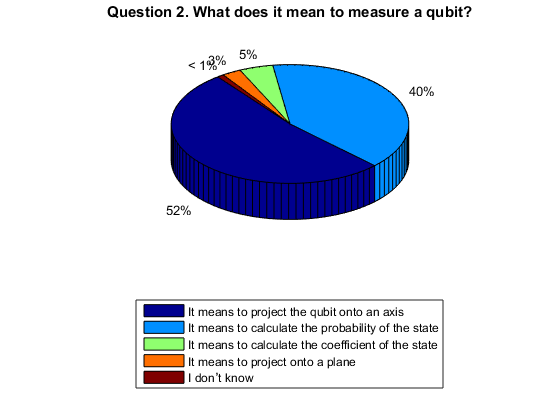
\includegraphics[width=0.45\textwidth]{E2P2_V1.png}}
    \\
     \subfloat{
   \label{fig:E2P3}
    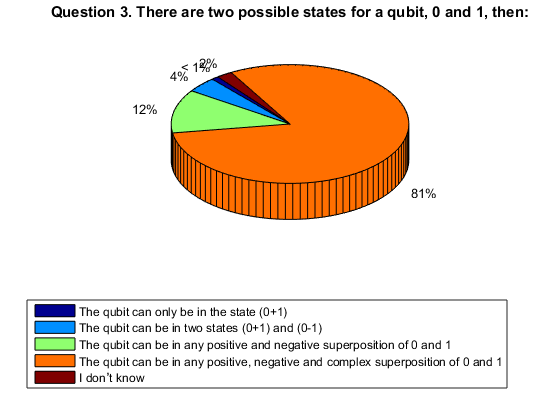
\includegraphics[width=0.45\textwidth]{E2P3_V1.png}}
     \subfloat{
   \label{fig:E2P4}
    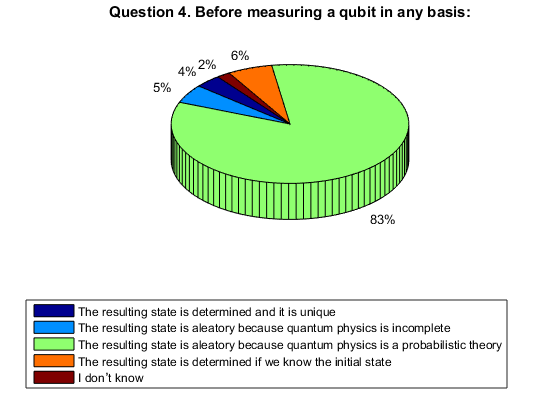
\includegraphics[width=0.45\textwidth]{E2P4_V1.png}}
    \\
    \subfloat{
   \label{fig:E2P5}
    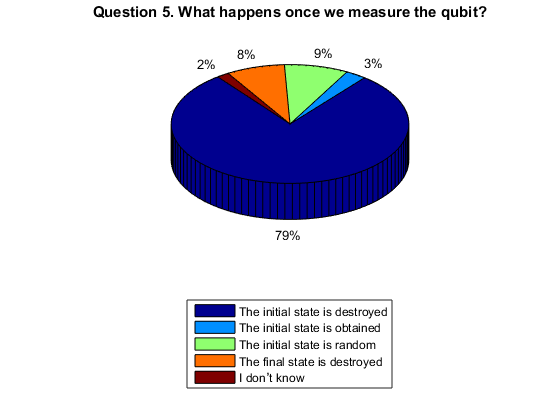
\includegraphics[width=0.45\textwidth]{E2P5_V1.png}}
     \subfloat{
   \label{fig:E2P6}
    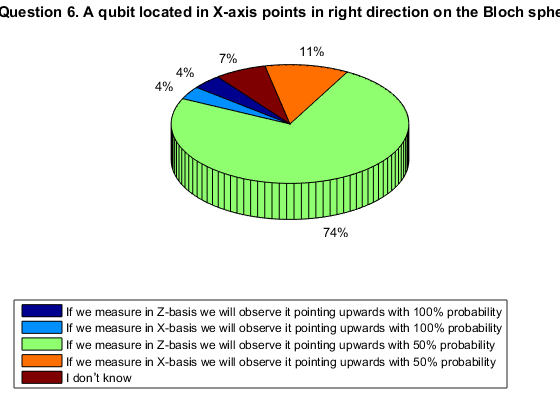
\includegraphics[width=0.45\textwidth]{E2P6_V1.png}}
    \\
     \subfloat{
   \label{fig:E2P7}
    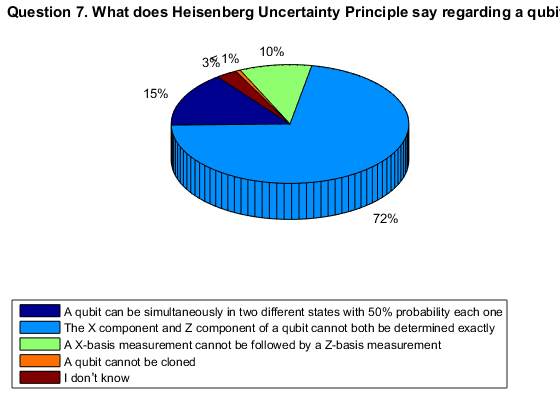
\includegraphics[width=0.45\textwidth]{E2P7_V1.png}}
     \caption{\footnotesize Answers Survey 2: After watching the video.}
 \label{fig:encuesta2}
\end{figure}


\begin{figure}[H]
 \centering
  \subfloat[]{
   \label{fig:GQ1}
    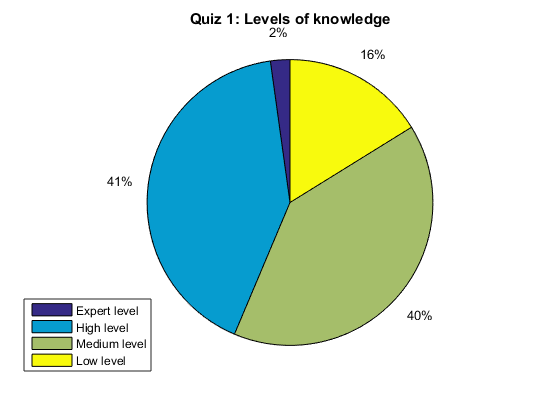
\includegraphics[width=0.5\textwidth]{GroupsQ1.png}}
  \subfloat[]{
   \label{fig:GQ2}
    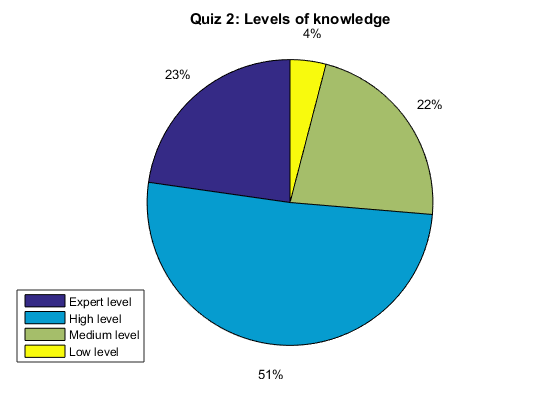
\includegraphics[width=0.5\textwidth]{GroupsQ2.png}}
    \caption{\footnotesize 4 Groups of differents levels of knowledge.}
 \label{fig:groups}
\end{figure}

\begin{figure}[H]
 \centering
  \subfloat[]{
   \label{fig:Exp}
    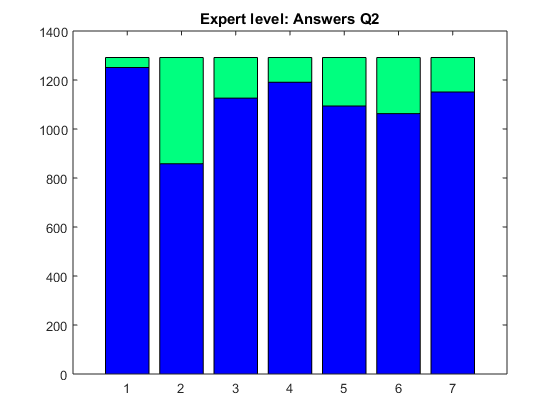
\includegraphics[width=0.5\textwidth]{ExpertQ2.png}}
  \subfloat[]{
   \label{fig:high}
    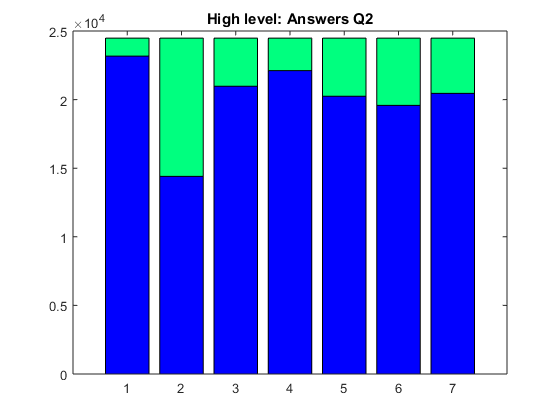
\includegraphics[width=0.5\textwidth]{HighQ2.png}}
    \\
    \subfloat[]{
   \label{fig:medium}
    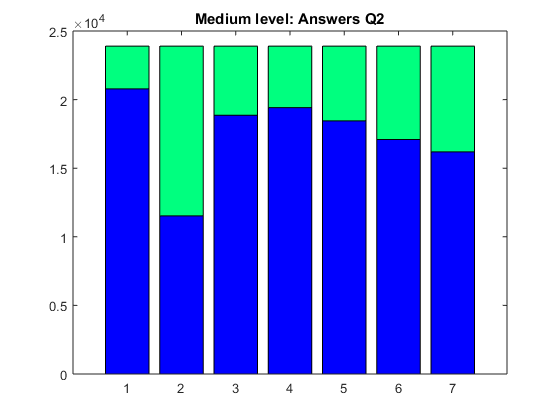
\includegraphics[width=0.5\textwidth]{MediumQ2.png}}
  \subfloat[]{
   \label{fig:low}
    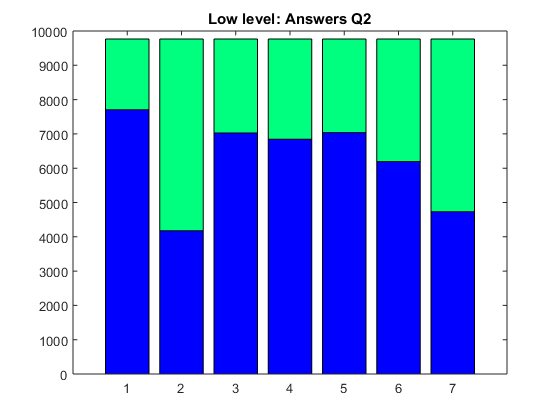
\includegraphics[width=0.5\textwidth]{LowQ2.png}}
    \caption{\footnotesize Answer to survey 2 of each group.}
 \label{fig:groupsQ2}
\end{figure}


\end{document}